\documentclass{article}
\usepackage{units}
\usepackage{booktabs}
\usepackage{graphicx}
\usepackage{amsmath, amsthm, amssymb, bm}
\usepackage{tikz, pgfplots}
\usetikzlibrary{shapes, arrows, positioning, fit, calc}
\newtheorem{theorem}{Theorem}
\newtheorem{Property}{Property}
\theoremstyle{remark}
\newtheorem*{defn}{Definition}
\renewcommand{\vec}[1]{\underline{#1}}
\usepackage{units}
\usepackage{fancyvrb}
\fvset{fontsize=\normalsize}

\title{AI1103 Assignement 1}
\author{Hritik Sarkar}

\begin{document}

\maketitle

PDF is given by  $f(x) = c e^{-x^{4}}, x\in \mathbb{R}$, where $ c = \frac{2}{\Gamma (\frac{1}{4})} $. What is the CDF ? \\
Answer: Gamma function $(\Gamma)$ is defined as 
\[
\Gamma (n) = \int_{0}^{\infty} e^{-x} x^{n-1} dx
\]

Similarly, upper incomplete Gamma function is defined as
\[
\Gamma (n,y) = \int_{y}^{\infty} e^{-x} x^{n-1} dx
\]

Cumulative Distribution Function $F$ for a Probability Density Function $f$ is defined as

\[
    F(y) = P(X\leq y) = \int_{-\infty}^{y} f(x) dx    
\]

\begin{itemize}

\item \large{Case 1: $y\geq 0$}

\begin{align*}
    I &= \int_{-\infty}^{y} c e^{-x^{4}} dx \\
    &= \int_{-\infty}^{0} c e^{-x^{4}} dx + \int_{0}^{y} c e^{-x^{4}} dx \\
    &= \int_{0}^{\infty} c e^{-x^{4}} dx + \int_{0}^{y} c e^{-x^{4}} dx \\
\end{align*}
\begin{align*}
  t&=x^4 \\
  \llap{$\Rightarrow$\hspace{50pt}} dt&=4x^3dx\\
  \llap{$\Rightarrow$\hspace{50pt}} dx &= \frac{1}{4} t^{-\frac{3}{4}} dt
\end{align*}

\begin{align*}
    I &= \int_{0}^{\infty} \frac{c}{4} e^{t} t^{(\frac{1}{4}-1)} dt + \int_{0}^{y^4} \frac{c}{4} e^{t} t^{(\frac{1}{4}-1)} dt\\
     &= \int_{0}^{\infty} \frac{c}{4} e^{t} t^{(\frac{1}{4}-1)} dt+ \int_{0}^{\infty} \frac{c}{4} e^{t} t^{(\frac{1}{4}-1)} dt - \int_{y^4}^{\infty} \frac{c}{4} e^{t} t^{(\frac{1}{4}-1)} dt\\
     &= \frac{c}{4} \Gamma(\frac{1}{4}) + \frac{c}{4} \Gamma(\frac{1}{4}) - \frac{c}{4} \Gamma(\frac{1}{4},y^4)\\
     &= \frac{c}{2}\Gamma(\frac{1}{4}) - \frac{c}{4} \Gamma(\frac{1}{4},y^4) \\
     &= 1 - \frac{c}{4} \Gamma(\frac{1}{4},y^4) &\textit{(substituting c)}
\end{align*}

\item \large{Case 2: $y < 0$}
\begin{align*}
    I &= \int_{-\infty}^{y} c e^{-x^{4}} dx \\
    &= \int_{{y}'}^{\infty} c e^{-x^{4}} dx &&\textit{(where {y}' = -y)}\\
    &= \int_{{y}'^4}^{\infty} \frac{c}{4} e^{t} t^{(\frac{1}{4}-1)} dt \\
    &= \frac{c}{4} \Gamma(\frac{1}{4},{y}'^4)
\end{align*}

\end{itemize}

So,
\[
    F(y)= 
\begin{cases}
    1 - \frac{c}{4} \Gamma(\frac{1}{4},y^4),& \text{if } y\geq 0\\ \\
    \frac{c}{4} \Gamma(\frac{1}{4},y^4)              & \text{otherwise}
\end{cases}
\]
\begin{figure}
    \centering
    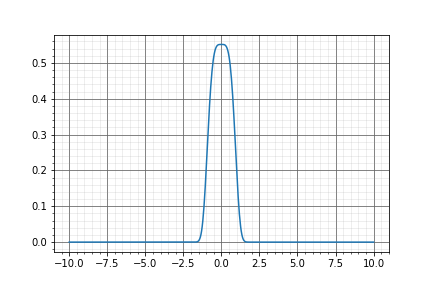
\includegraphics[scale=0.75]{PDF.png}
    \caption{Plot of the PDF}
    \label{fig:my_label}
\end{figure}

\end{document}